\documentclass[main.tex]{subfiles}

\begin{document}
\chapter{Concept Design}
\chaplabel{conceptDesign}
Various concept designs for each system are required to ensure that the optimal design can be developed for each system. This chapter will discuss the various designs and software configurations considered. Decision matrices were utilised to pick the most appropriate system.
\section{Platform Selection}
\seclabel{platformselect}
A platform is used as a means to mount the required detection equipment and to act as the foundation for a completely autonomous system.  Design and construction of the platform is not in the scope of the project and so the modification of an existing platform was the preferred approach. The selected platforms included in the decision process were based directly on their availability to the project, whether a commercial product or the loan of equipment. Primary factors that were considered during the selection process were taken from the Project Specifications (see \secref{performance}) and the Project Scope (see \secref{projectScope}). The following list outlines the discussion points for each of the platform subsections:
\begin{itemize}
\item Cost: Based on a budget of \$16,500. A platform cost nearing \$5,000 indicated that the requirement had been met. A score of 10 indicates platform supplied in-kind and 1 indicates financially infeasible.
\item Implementation of Auto-Control: How involved the process of implementing the direct hardware required for remote operation would be. A low score indicates a difficult process with many sub-systems, whereas a high score indicates little to no work necessary. Requirement was met if implementation of hardware was a feasible task.
\item Control/Manoeuvrability: How appropriate the platform was expected to be regarding manoeuvrability assuming auto-control was implemented successfully. This included speed, acceleration, turn radius, and stopping distance.
\item Implementation of detection equipment: Ease of installation of detection equipment and expected effectiveness of the platform and sensor combination from a landmine detection point of view.
\item Payload: Platform's ability to support the required 100 kg payload.
\item Terrain Traversing: How capable the platform is at traversing the required terrain. This includes dry and loose sand or gravel with minimum obstacles and a 15 degree gradient.
\item Portability: Level of portability. A higher score indicates simpler transport with less disassembly required. The requirement had been satisfied if transport was possible in the back of a ute or trailer.
\item Navigation: How direct and efficient the path of the platform for mine-detecting purposes was expected to be. This involves aspects such as duration and tightness of turns and mine avoidance techniques.
\end{itemize}

\subsection{Utility Quad Bike}
Quad bikes are designed as all terrain vehicles and are capable of traversing even the most demanding terrains. Utility quad bikes are intended to carry large loads as well as a human operator and so load limits are frequently larger than 100 kg. Due to the nature of the platform and through visual inspection, mounting points for sensor brackets and electronic systems are located in various positions.  Environmental conditions are of little concern to this platform which will be encountered and traversed with ease for ranges of over 100 km. Turning radius for quad bikes are typically in the range of 3-4 metres.
The DSTG have offered the use of one of their autonomous quad bikes to be used as the platform. The DSTG quad bike is a Honda TRX450r and has a weight load capacity of 110 kg. The quad bike has been previously fitted with remote control capabilities and is in good working condition, however \textcite{scheiner2011} recommended that the brake actuator be replaced as well as some electronics. As the platform already has remote control capabilities, transport becomes a much easier task especially with a trailer or ute with a ramp.
\begin{figure}[ht]
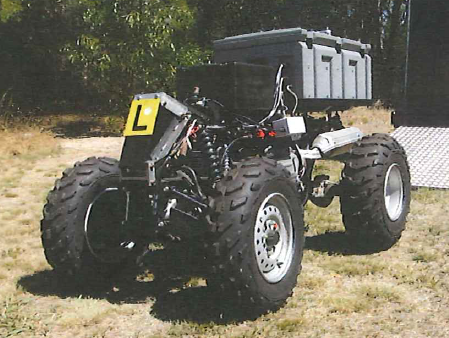
\includegraphics[width=0.4\textwidth]{4-ConceptDesign/2011quadbike.PNG}
\centering
\caption[DSTG Autonomous Quad Bike]{DSTG Autonomous Quad Bike \parencite{scheiner2011}} \figlabel{2011quadbike}
\end{figure}

\subsection{Dune Buggy}
A dune buggy is vehicle designed for high speed operation on loose, sandy terrain. Design of dune buggies are commonly an open chassis housing a modified vehicle and thus it's performance characteristics are similar or better than that of a small car. They are commonly able to carry two persons resulting in a load capacity exceeding 160 kg. Dune buggies frequently have turn radii around 6 metres restricting path curvature for accurate tracking. Due to the nature of the platform equipment mounting is common practice and would not raise any issues however a bare mass of 230 kg and dimensions 2.3 x 1.5 metres would make the unit difficult to transport.
\begin{figure}[ht]
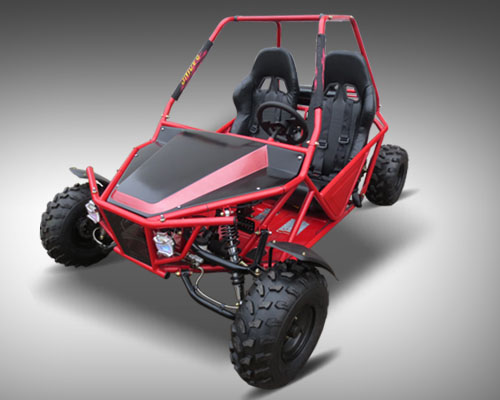
\includegraphics[width=0.4\textwidth]{4-ConceptDesign/kandidunebuggy.jpg}
\centering
\caption[Example of dune buggy - Kandi-150]{Example of dune buggy - Kandi-150 \parencite{150GKM}} \figlabel{kandi150}
\end{figure}

\subsection{Continuous Track Vehicle}
Tracked vehicles are designed to distribute the weight of the vehicle over a large area enabling the traversing of soft and loose terrain without the concern of losing traction and becoming stuck. The platform shown in \Figref{grillon500} is one example of such a vehicle. The Grillon-500 is able to carry a payload of 1000 kg and operate at speeds up to 11 km/hr however a bare mass of 100 kg and dimensions of 1.5 m by 2.5 m could make the unit difficult to transport \parencite{cinamGrillon}. This model is designed to support the mounting of various equipment in the front bay (fork lift pictured). An advantage of the tracked vehicle over other platforms is its ability to turn on the spot eliminating the need for complicated turn algorithms. 
\begin{figure}[ht]
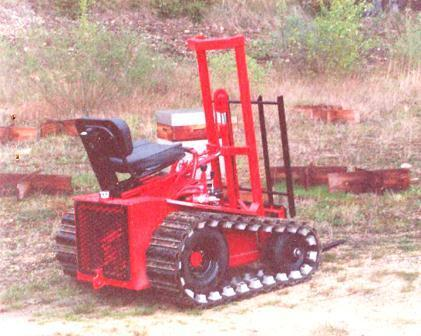
\includegraphics[width=0.4\textwidth]{4-ConceptDesign/Grillon-500.jpg}
\centering
\caption[Example of tracked vehicle - Grillon-500]{Example of tracked vehicle - Grillon-500 \parencite{cinamGrillon}} \figlabel{grillon500}
\end{figure}

\subsection{Hovercraft}
Access was made available to an existing hovercraft from a 2009 Adelaide University Honours Project. Analysis of the technical report \parencite{hovercraft2009} and practical and theoretical evaluations showed that the lift fan was able to support a payload of up to 22 kg and the thrust fans were only just capable of moving the craft on a flat, smooth surface. For complete automation only actuators for the lift motor would be required as remote operation for the thrust system had already been implemented. The stopping distance is lacking due to the time required to rotate fans for reverse thrust. The hovercraft has an advantage over other platforms through its ability to pass directly over a mine without detonation occurring, however, this 'sliding' advantage introduces new problems when developing a path tracking algorithm due to the advanced dynamics of the platform. The purchasing of a recreational hovercraft more suited to the requirements would not have been financially feasible. Through verbal discussion with DSTG, it was revealed that vibrations produced through the lift and thrust systems on hovercraft platforms were detrimental to the effectiveness of the sensor equipment. Thus, the DSTG has advised against the use of a hovercraft as the platform for mine-detecting purposes.
\begin{figure}[ht]
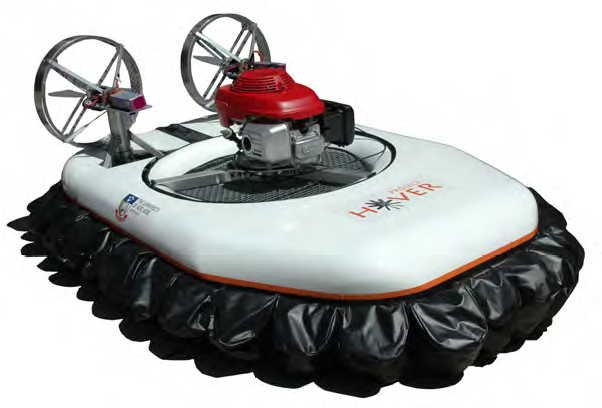
\includegraphics[width=0.4\textwidth]{4-ConceptDesign/HovercraftPic.png}
\centering
\caption[2009 Adelaide University Honours Project Hovercraft]{2009 Adelaide University Honours Project Hovercraft \parencite{hovercraft2009}} \figlabel{hovercraftPic}
\end{figure}

\subsection{Platform Decision}
\Tabref{platformDecision} summarises the strengths of each of the considered platforms. A score of 5 indicated that a requirement had been satisfied or that the criterion was only just feasible for that platform, with any difference being representative of a rise or fall in the platforms specified capability. Scores had a lower limit of 1 and an upper limit of 10. It was evident that the hovercraft did not meet majority of the requirements to be the supporting platform. Commercial quad bikes or dune buggies could have been used with some modifications to the structure, however a tracked vehicle or the quad bike offered by DSTG were clearly the two best options.

The DSTG quad bike was selected over a tracked vehicle for a number of reasons. These included direct availability, financial restrictions, and the completed state of auto control hardware already on the quad bike.
\begin{table}[ht]
\centering
\caption{Platform decision matrix}
\tablabel{platformDecision}
\begin{tabular}{r *6c}
    \multicolumn{1}{r}{}  & \mcrot{1}{l}{45}{Hovercraft (2009)} & \mcrot{1}{l}{45}{Commercial Quad Bike} & \mcrot{1}{l}{45}{Dune Buggy} & \mcrot{1}{l}{45}{Tracked Vehicle} & \mcrot{1}{l}{45}{Quad Bike (DSTG)}\\ \toprule 
    Unit Cost & 10 & 5 & 3 & 4 & 10\\ 
    Implementation of Auto Control & 5 & 3 & 3 & 5 & 9\\ 
    Control/Manoeuvrability & 3 & 7 & 5 & 9 & 7\\ 
    Implementation of Detection Equipment & 1 & 6 & 6 & 5 & 6\\ 
    Payload & 2 & 8 & 10 & 7 & 7\\ 
    Terrain Traversibility & 3 & 9 & 7 & 10 & 9\\ 
    Portability & 7 & 6 & 4 & 8 & 6\\ 
    Navigation & 9 & 5 & 4 & 7 & 5\\ \midrule
    \textbf{Total} & 48\% & 64\% & 57\% & 68\% & 76\%\\ \bottomrule
\end{tabular}
\end{table}

\section{Navigation and Automation}
The navigation and automation systems are responsible for communicating to the quad bike two primary functions, how to follow a path and what quad bike control elements need to do to allow this to happen. Platform navigation will be primarily handled via waypoints. After a region is selected by a user it is broken down into a series of waypoints which, once connected, will form a path for the quad bike. In the alternate use case, the navigation system will operate based directly on waypoints created from a user defined path.

\subsection{Path Tracking}
\seclabel{pathconcept}
As the platform will be primarily performing two tasks, following a low curvature curve (straight line) and turning a specified angle, the navigation system will define the path using a 'piecewise linear path' discussed in \secref{pathTrackingLitReview}. \Textcite{snider2009} provides an empirical comparison of path following algorithms and is shown in \Figref{trackingComparison}. Tracking methods are ordered by implementation difficulty from least difficult to most difficult. \Textcite{snider2009} goes on to describe recommended applications for each method.  Pure pursuit is ideal in situations for slow driving and/or on discontinuous paths, the Stanley method for smooth highway driving and/or parking manoeuvres, the Kinematic model for smooth parking manoeuvres, and the Dynamic model for highway driving at speed. The most suited to the landmine detection application is slow driving on discontinuous paths and thus Pure Pursuit will be used as the tracking method.
\begin{figure}[ht]
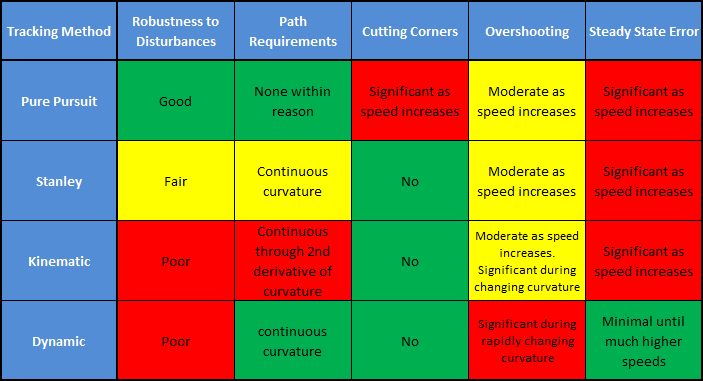
\includegraphics[width = \textwidth]{4-ConceptDesign/pathTrackingSummary2.png}
\centering
\caption[Empirical Comparison of Path Tracking Algorithms]{Empirical Comparison of Path Tracking Algorithms \parencite{snider2009}} \figlabel{trackingComparison}
\end{figure}

\subsection{Turning the Platform a Specified Angle}
At the end of a swathe the platform will be required to turn a specified angle within a small area defined by the width of the sensing arrays. Alternatively, if the scan history is available to the platform in the form of a map, a larger area may be available to conduct the turn. Due to little or no literature on the unique topic an adaptation of the simplified Ackermann model will be used in conjunction with the Stanley model (good for parking manoeuvres) to achieve the desired turn.

\subsection{Platform Automation}
\seclabel{automationconcept}
The automation of the quadbike selected from \secref{platformselect} may be modelled using the input parameters from the PID controller discussed in \secref{autocontrol}. The flow chart design for the quad bike control is shown in \Figref{autoflowchart} and enables transfer to various programming languages, such as, Matlab, C++ and Java. \Figref{autoflowchart} shows that the PID controller processes the four different input functions as described in \secref{autocontrol}. The result is transmitted back to the actuators, the output window and central hub. The window is used as a visual output of the current conditions of the quad bike. The central hub processes the overall integration of the system and links this autonomous control to the navigation, which is discussed further in \secref{conceptprojectdesign}. 

\begin{figure}[ht]
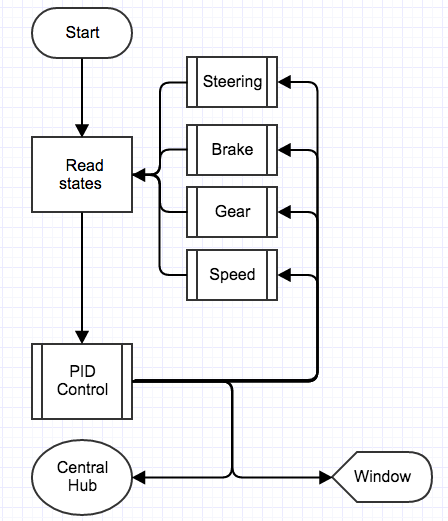
\includegraphics[width=0.6\textwidth]{4-ConceptDesign/autoflowchart.png}
\centering
\caption{Platform automation flow chart} 
\figlabel{autoflowchart}
\end{figure}

The automation software includes the main input parameters from \secref{autocontrol}. \Figref{autocode} shows that the functions have different processes implemented under each one, with an additional function called emergency stop to be included for safety purposes. This emergency stop function will interrupt all processes if the operator deems it necessary. The specific process under each main function is the "get" and "set" processes. The "get" process is to read the current state of the actuator or servo motor, and the "set" process is to save that current state and expected values in order to calculate the relevant error. There will be further processes added to automate the platform and integrate the navigation path tracking and turning sections.

\begin{figure}[ht]
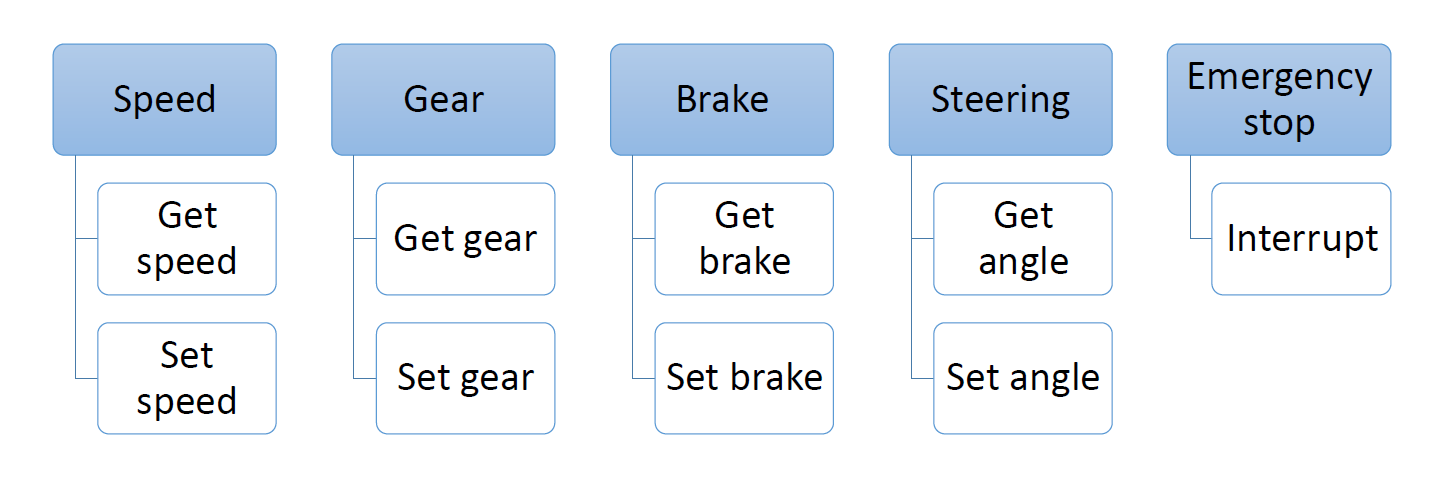
\includegraphics[width=\textwidth]{4-ConceptDesign/autofunct.PNG}
\centering
\caption{Automation code functions} 
\figlabel{autocode}
\end{figure}

\section{Signal Processing}
\seclabel{signalconcept}
As noted in \secref{gpr}, the detection depth and resolution are generally fixed parameters of the transmitting and receiving antennas of the physical device. The signal processing software will be designed to operate effectively on the hardware available, which is the GPR unit supplied to the project courtesy of the DSTG. The model is a single GPR (non-array) unit with three interchangeable antennas which allow the selection of transmission and receiving frequency. The three heads supplied are:
\begin{itemize}
\item 800 MHz
\item 1.4 GHz
\item 2.0 GHz
\end{itemize}
During the course of the project a single antenna head will be used, determined by initial testing to be the frequency which generates the highest resolution data while providing depth of scanning as required by the project goals. A suitable metal detecting unit will be sourced from commercially available systems to match the detection range of the GPR unit supplied, to provide the greatest overlap of scanning capacity.
The software and systems developed will be generated as a proof-of-concept using the initial available equipment, with considerations made to allow for simple expansion to array based detectors for the benefits discussed in \secref{gpr}. 

In consideration of the project timeframe and expected capacity of group members, the proposed signal processing system will seek to employ a Decision-level Sensor Fusion strategy to improve the detection and false-positive error rates over that of the individual sensors. This is expected to be achieveable and will demonstrate the core abilities of the sensor fusion strategy to improve detector classification. \\

The decision-level sensor fusion becomes more accurate with more decision metrics available about the object. To make the most of the sensors available to the platform, the following decisions metrics will be used as inputs to the sensor fusion stage:
\begin{itemize}
\item Inverse-matched filter from a single GPR sample (Ascan)
\item Hyperbola detection from a collection of GPR samples (Bscan)
\item Phase plot signature matching from a single metal detector sample
\end{itemize}
Each individual determination of likelihood that an object can be classified as a mine will be based around an individual scan's similarity to a training data set, produced from testing data. The final determination of the likelihood that an object is a mine will be based upon a linear weighting of the three metrics, offset by the relative confidence in each decision metric. Time permitting, the training data sets and the weighting coefficients will be generated from the output of an artificial intelligence machine learning algorithm based on decision trees, neural networks or fuzzy logic. Initially the trained data sets and weighting coefficients will be manually trained by inspection.

\section{Electronics}
Requirements for the electronics subsystems can be inferred from the project aims. As a major component of the project would be attempting advanced signal processing methods in real time, significant processing capabilities will be required on the mobile platform. In addition to this, the signal processing must be capable of running simultaneously with a number of other platform software systems, such as vehicle control and telemetry. To achieve this without requiring multiple discrete hardware components (which would require communications input/output (I/O) interfaces to share data), a single hardware system capable of executing multiple threads simultaneously and asynchronously is required on the vehicle. The hardware system executing the signal processing software must also be capable of reading sensory input from USB devices, as this is the communications format available on the GPR units provided by the DTSG. 
\nomenclature[A]{I/O}{Input/Output}% 

A second major component of the project is the automation of the remote vehicle, requiring software control over a series of actuators and sensors. To provide the greatest fidelity of control over the vehicle the electronics hardware used to interface with the actuators and sensors must be capable of reading and writing to low-level I/O devices quickly and with minimal latency or overhead. To achieve this, the ability to create hardware interrupts are desirable, which would allow the software to process incoming sensory data as soon as it is received. The software for the parsing and decoding of raw input signals to generate usable information is not expected to be complicated, as so the hardware will not need to be particularly advanced or have capacity for high speed processing.

\begin{itemize}
\item \textbf{Bespoke Electronics}\\
Bespoke electronic equipment has the capacity to allow incredibly fast access to I/O devices through the use of task-specific commercial off-the-shelf (COTS) chips. However, the time consumption and expense of planning an entirely hardware-driven control system for anything more than trivial data handling is inappropriate for this project. The inability to prototype as with software means that the ability to test and then revisit a solution is not possible, and a hardware/purely electronics driven system is not capable of general purpose processing. Therefore, this is not a realistic option for achieving the project aims.
\nomenclature[A]{COTS}{Commercial Off-The-Shelf}% 
\item \textbf{Microcontrollers}\\
Microcontrollers have become the de facto standard for small to medium software-based projects which require access to physical sensors and actuators, due to their readily available access to low level I/O. Microcontrollers supporting common languages such as C++ and Java allow easy development and rapid prototyping, though the inability to easily connect debugging equipment or generate test output slows the development process. Microcontrollers are inexpensive and provide high I/O availability but at the cost of limited processing power. The low-level nature of microcontrollers means that desirable features like hardware interrupts are exposed to and accessible by developers. 
\item \textbf{Desktop computing equipment/Laptop} \\
Conventional desktop computing equipment is the fastest general purpose computing hardware that will be available to the project. In addition to having the greatest computing power, it has the highest ability to support prototyping and allows for rapid software development with readily accessible software generation and debugging tools. The drawback of this higher-level computing platform is the reduced accessibility of low-level I/O devices, and the amount of computing overhead caused by operating system processes. Operations that require fast I/O access may be hampered by the inability to ensure thread availability, and so for robust operation this may require buffering to a secondary, lower level device.
\end{itemize}

None of the individual items presented allow for the full range of requirements of this project. As a result, the general concept for the hardware arrangement to execute the software systems is shown below in \Figref{hardwareLayout}.
% is this figure text fucking big enough maziar??
\begin{figure}[ht]
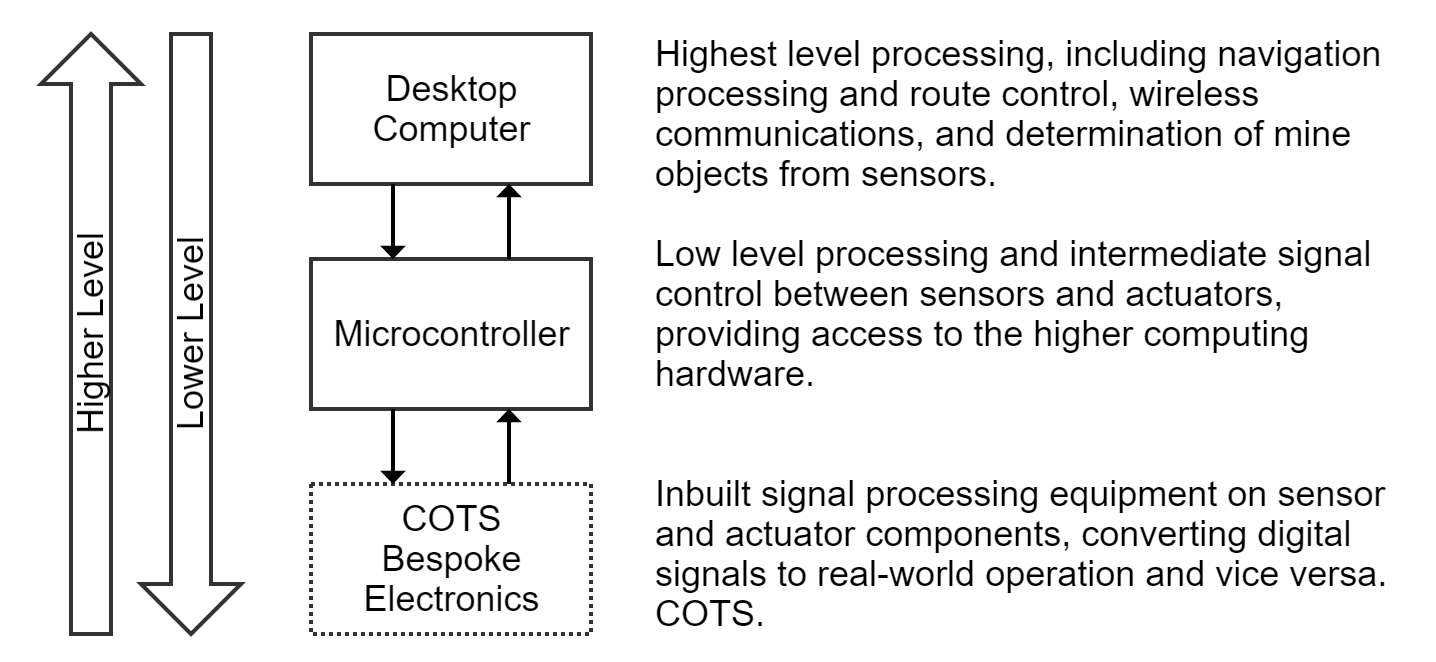
\includegraphics[width = \textwidth]{4-ConceptDesign/electronics.png}
\centering
\caption{Conceptual Hardware layout} \figlabel{hardwareLayout}
\end{figure}

Under this system, the project will use standard desktop computing equipment for the bulk of the software, to make use of its superior processing power and the rapid development it allows. This device will be the data handler and processor, and act as the 'central' software location for the project. Sensors and actuators that require low level I/O access will be connected to a secondary microcontroller, which will act independently to buffer inputs and outputs of the system, which can then be communicated to the primary computer over a serial communications connection. The project will not aim to develop any custom electronics boards and handle all signal amplification or processing in software.

\section{Sensor Mount}
\seclabel{sensormount}
The sensor mount is required to support the weight of both the GPR and the metal detector as well as be sturdy enough to prevent flexing or warping during operation. The following section describes the basic requirements imposed on the mount.  
\subsection {Sensor Requirements } 
The design of the mount must satisfy the performance requirements of each sensor. These include the sensors operating height off the ground and their optimal operating distance from other objects to prevent interference. 

Both the GPR and metal detector must operate horizontally and within close proximity to the ground to ensure no erroneous data.
For minimal ground reflections and interferences, the GPR should operate as close to the ground as possible. Optimal operating conditions for the GPR requires ground contact to trigger the scroll wheel switch. Sensitivity tests to objects above and beside the GPR resulted in little interference. Objects above 50mm had no impact on the data as well as objects 100mm beside it. 

The metal detector is more sensitive to metallic objects above and beside it. A stand-off distance for metallic objects of 500mm is required as well as a vertical stand-off distance of 2 meters. To reduce size, the GPR will be closest to the platform with the metal detector in front, allowing for the required stand-off distance.  
\subsection {Material Selection}  
Material selection is largely dependent on the sensor requirements as well as taking into consideration its ease of sourcing, working and repairing. Non metal structures are required due to the metal detector therefore, possible material choices include PVC piping, carbon fibre, wood and fibreglass. \Tabref{sensorMountMaterials} represents decision matrix used to determine the material for the mount.

\begin{table}[ht]
\centering
\caption{Sensor mount material selection matrix}
\tablabel{sensorMountMaterials}
\begin{tabular}{r *4c}
    \multicolumn{1}{r}{}  & \mcrot{1}{l}{45}{\textbf{PVC}} & \mcrot{1}{l}{45}{\textbf{Carbon Fibre}} & \mcrot{1}{l}{45}{\textbf{Wood}} & \mcrot{1}{l}{45}{\textbf{Fibreglass}}\\ \toprule 
    Cost & 10 & 1 & 10 & 3 \\ 
    Ease of manufacture & 10 & 1 & 5 & 3 \\ 
    Ease of repair & 10 & 4 & 8 & 5 \\ 
    Ease to source & 10 & 2 & 10 & 6 \\ 
    Time to build & 10 & 1 & 8 & 10 \\ 
    Strength & 5 & 10 & 6 & 7 \\ \midrule
    \textbf{Total} & 92\% & 32\% & 78\% & 57\% \\ \bottomrule
\end{tabular}
\end{table}

PVC scored the highest due to its low cost, ease to modify and ease of assembly. However, it is not the strongest material and could flex during operation depending on the length.
Carbon fibre is the strongest material but the cost and hardships associated with it resulted in the lowest score. Wood is the second highest but the joining of sections without nails would result in weaker joins. Fibreglass scored in the middle primarily due to the cost and difficulties to manufacture. 
PVC will be used for the primary arm of the supporting bracket holding the metal detector. As strength has been identified as an issue from the selection matrix, future discussions with workshop staff as to the ability to source the required thicknesses to meet the strength criteria, or for the manufacturability of bracing and reinforcement for PVC parts.

%\textcolor{red}{havnt explicitly stated what material we will be using. obviously PVC but then need to offer a solution to the strength issue that comes with PVC. also would it be possible to have metal supporting the gpr then pvc coming off of that to help with the strength issue} 
%% ^^ harry if you want to extend this disucssion still then feel free. but until then i've removed the comment just to clean everything up

\subsection{Sensor Mount Design}
Basic design for the sensor mount can be realised with the sensor requirements. Using the DSTG Quad bike as the chosen platform, preliminary designs can be sketched. Considerations for both front and rear mounted sensor arrays were considered. Design 1, 2 and 3 trial different mounting techniques and frame designs.



\subsubsection{Design 1}
Design one is represented in \Figref{design1} and is a rear mounted frame. This mount assumes that the quad bike will be more manoeuvrable when steered from the rear, requiring the direction of travel to be in reverse. Thus, the frame mounting on the back is necessary. 
 \begin{figure}[ht]
 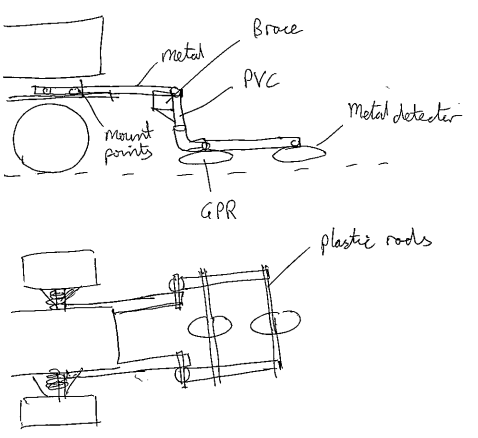
\includegraphics[width=.5\textwidth]{4-ConceptDesign/Rear_Mount.png}
 \centering
 \caption{Design 1 Rear frame mount}
 \figlabel{design1}
 \end{figure}

\subsubsection{Design 2}
Design 2 represents a front mounted frame assuming that the quad bike is driven in a standard configuration as shown in \Figref{design2}. The GPR is placed in close proximity to the body with the metal detector attached further in front. This design appears to be the smallest and use the least amount of material.
\begin{figure}[ht]
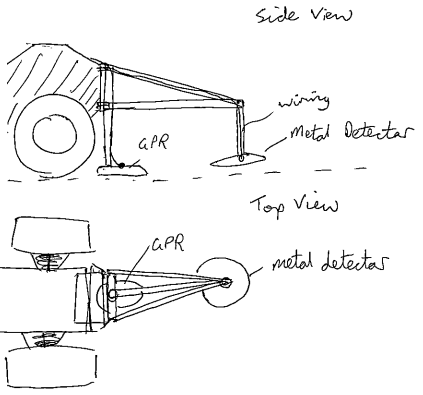
\includegraphics[width=0.5\textwidth]{4-ConceptDesign/front_frame_design_triangle.png}
\centering
\caption{Design 2 Front frame mount}
\figlabel{design2}
\end{figure}
\subsubsection{Design 3}
Design 3 incorporates a staggered design with the metal detector and GPR placed further in front of the platform as shown in \Figref{design3}. This larger stand off distance would allow for less violent stops as the allowable stopping distance would be increased. However, the required material and weight would be greater potentially requiring greater reinforcements to mitigate flexing and warping. These reinforcements could be from the use of fibreglass coating over the PVC piping.
\begin{figure}[ht]
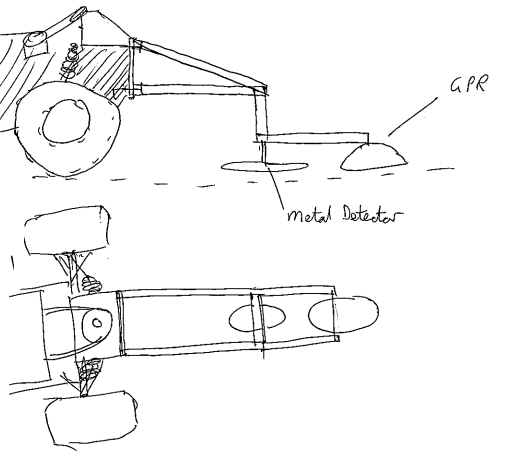
\includegraphics[width=0.5\textwidth]{4-ConceptDesign/front_mount_staggered.png}
\centering
\caption{Design 3 Front frame mount}
\figlabel{design3}
\end{figure}\\

The sensor mount will be made from a combination of PVC and fibreglass. The fibreglass will be supporting sections to prevent flexing and warping. As exact dimensions and platform performance characteristics are unknown, specific mounting orientation and size cannot be decided upon until the platform is delivered. Once the Platform has been delivered for the project, specific and more detailed designs can be created

\section{Conceptual Project Design}

\seclabel{conceptprojectdesign}
\begin{figure}[ht]
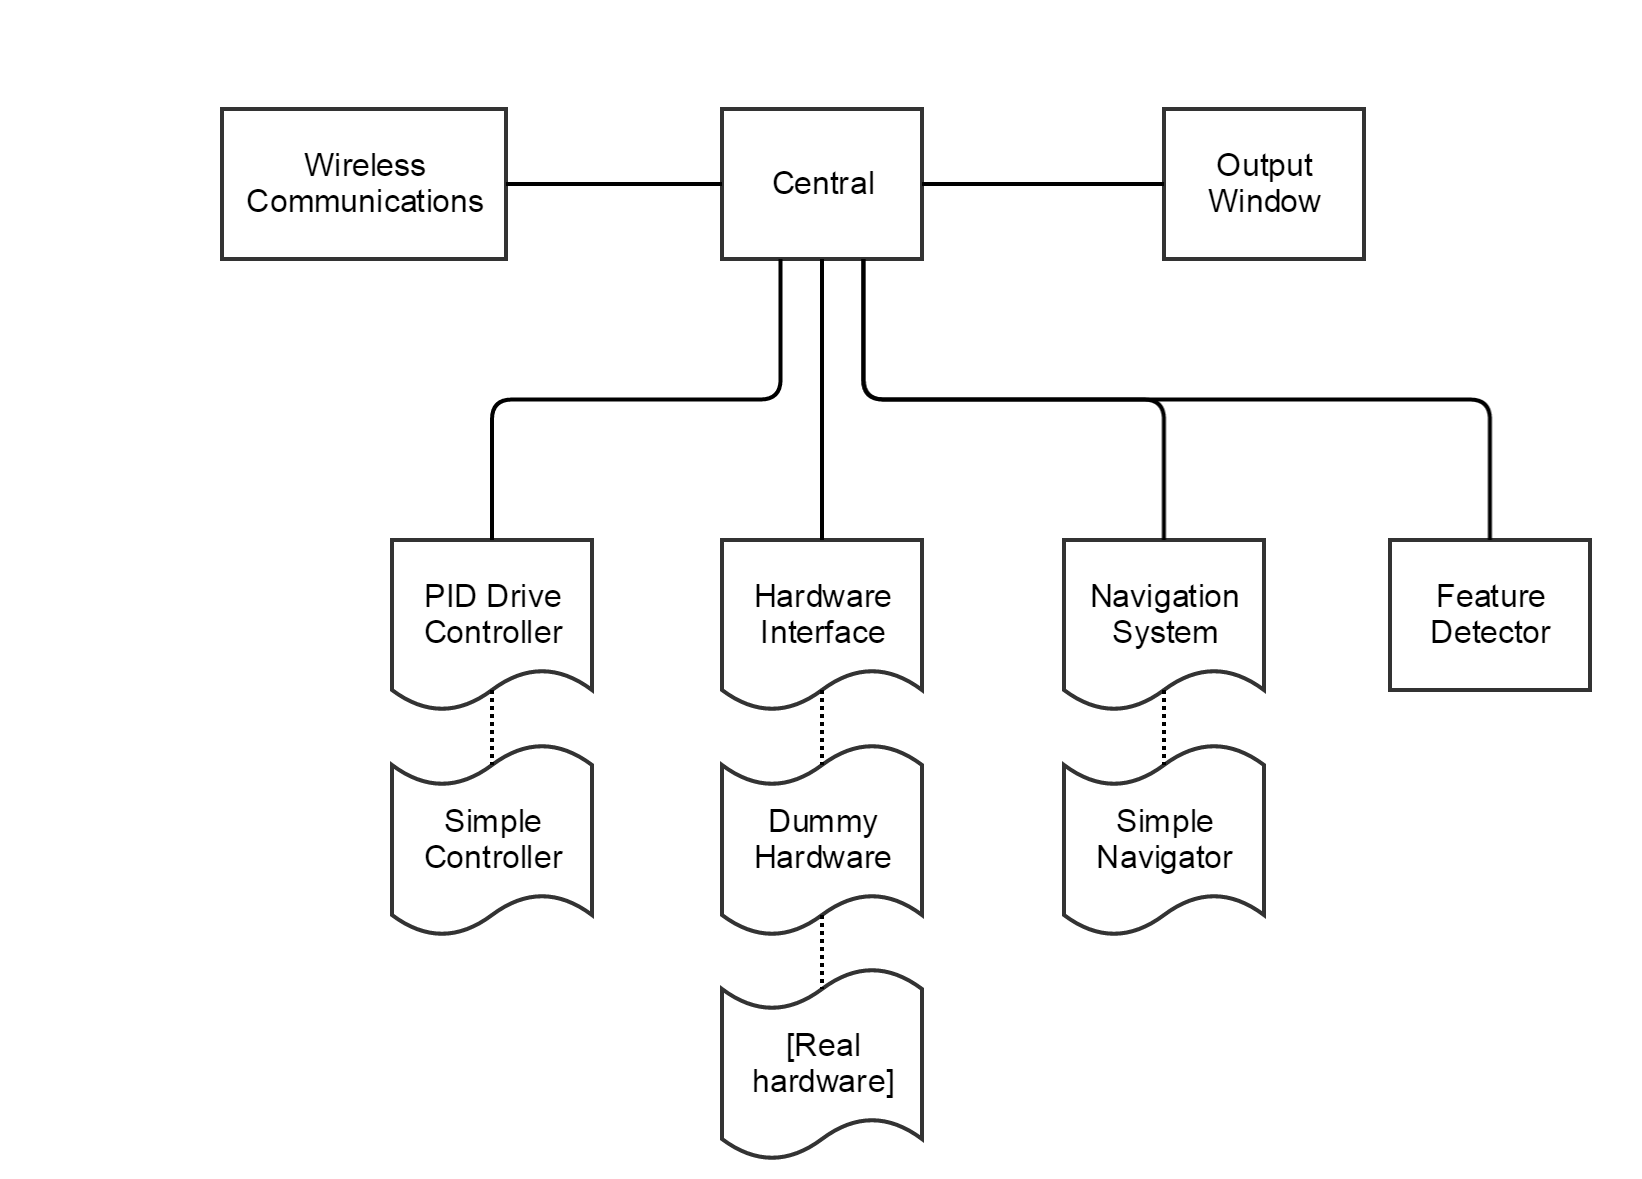
\includegraphics[width=\textwidth]{4-ConceptDesign/fyp_structure.png}
\centering
\caption{Integration of automation, navigation, sensors and signal processing} 
\figlabel{central}
\end{figure}

The autonomous quad bike will be used as the platform on which the sensor mount and software subsytems will operate. A concept is shown in \Figref{frontConcept} and \Figref{rearConcept}. To achieve the framework for overall automation of the platform the integration of the actuator electronics, navigation, sensors, signal processing and operator device is required. This framework is completed through the Central Hub as shown in \Figref{central} where dotted lines indicate implementations of the interfaces. The Central Hub will combine and read all the relevant processes and transmit the required information to the operator device. This enables all processes to be completed in parallel, satisfying the deliverables as defined in \secref{primary}.

\begin{figure}[ht]
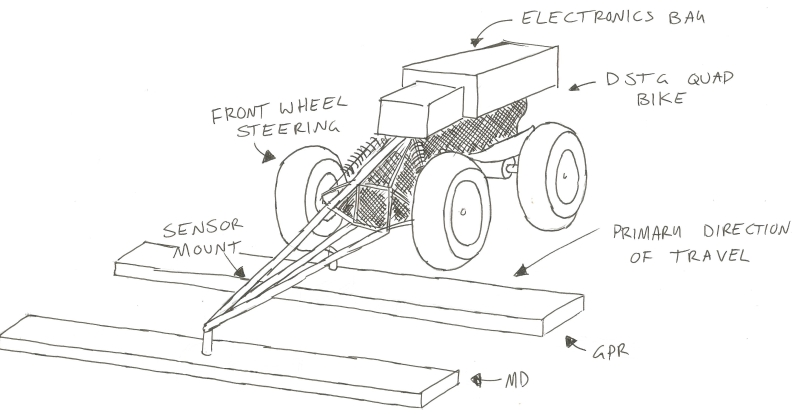
\includegraphics[width = 0.8\textwidth]{4-ConceptDesign/ConceptFront.jpeg}
\centering
\caption{Front wheel drive platform concept design} \figlabel{frontConcept}
\end{figure}
\begin{figure}[ht]
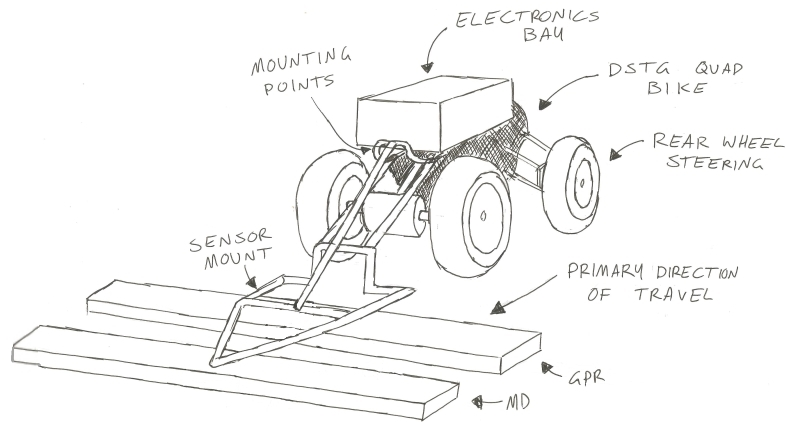
\includegraphics[width = 0.8\textwidth]{4-ConceptDesign/ConceptRear.jpeg}
\centering
\caption{Rear wheel drive platform concept design} \figlabel{rearConcept}
\end{figure}

The DSTG quad bike provides a basis to apply the completed concept designs and build upon them in order to have detailed designs for the automation and signal processing. 

\end{document}